\documentclass[a4paper,twoside]{article}
\usepackage[a4paper, total={6in, 10in}, bindingoffset=8mm]{geometry}
\usepackage{titletoc}
\usepackage{xstring}
\usepackage{textcomp}
\usepackage[hidelinks]{hyperref}
\usepackage{color}
\usepackage{titlesec}
\usepackage{graphicx}

%\makeatletter
%\let\latexl@section\l@section
%\def\l@section#1#2{\begingroup\let\numberline\@gobble\latexl@section{#1}{#2}\endgroup}
%\makeatother

% non-page-breaking line break
\newcommand*{\NLS}{%
	\par
	\nobreak
	\vspace{-\parskip}%
	\noindent
	\ignorespaces
}


\newcommand{\songheading}[2]{
	%\vbox
	~\\
}

\newcommand{\song}[3]{
	\songheading{#1}{#2}
	~\NLS
	#3
	%\titlespacing*{\section}{0pt}{1.5cm}{0.4cm}
	\vspace{1cm}
	%~\\~\\~\\
}

\definecolor{codebgcolor}{gray}{0.3}
\newcommand{\songWithoutText}[2]{
	% option 1: Just the entry in the TOC, but not between the texts anymore
	%\addtocontents{toc}{\vspace{0.4cm} \hspace{-0.55cm}\textbf{#1} ~\NLS #2\hfill {\color{codebgcolor}\texttimes}\par}
	
	% option 2: entry in TOC and between the lyrics
	\songheading{#1}{#2}
	\vspace{1cm}
	%\titlespacing*{\section}{0pt}{1cm}{0.4cm}
}


\usepackage{etoolbox}
\usepackage{tikz}
\newcommand\drawukulelechord[2][]{%
	\edef\chord{#2}%
	\begin{tikzpicture}[x=1.45ex,y=2ex,line cap=round,line width=.4pt,
	baseline=(current bounding box.center),#1]
	\draw[line width=.6pt] (1,0) -- (4,0);
	\foreach \d in {1,...,4}{\draw (1,-\d) -- (4,-\d);}
	\foreach \d[count=\p] in \chord {
		\draw (\p,0) -- (\p,-4.8);
		\ifdefstring{\d}{-1}{
			\draw (\p,.25) +(-.125,-.125) -- +(.125,.125)
			+(-.125,.125) -- +(.125,-.125);
		}{
		\ifdefstring{\d}{0}{
			%\draw (\p,.25) circle(.125); % opened string
		}{
		\fill (\p,.5-1*\d) circle(.25);
	}
}
}
\path[use as bounding box] (0.5,.5) rectangle (4.5,-5);
\end{tikzpicture}%
}
\makeatletter
\newcommand\defineukulelechord[2]{%
	\csdef{@ukulelechord@#1}{\drawukulelechord{#2}}%
}
\newcommand\ukulelechord[1]{%
	\ifcsdef{@ukulelechord@#1}{%
		\csuse{@ukulelechord@#1}%
	}{%
	\GenericError{}{Undefined ukulele chord '#1'}{}{}% 
}%
}
\makeatother


\begin{document}
	
\renewcommand{\contentsname}{\centerline{Ukulele songs by Erik}}
\tableofcontents

%\cleardoublepage
\clearpage

\twocolumn
\setlength{\columnwidth}{0.85\linewidth}

\titlespacing*{\section}{0pt}{0cm}{0.4cm}
% This file was automatically generated by the updateSongs - script
% and will get overwritten by it again. Do not modify it!

\song{A-Team}{C CG $\mid$ C CG $\mid$ a aF $\mid$ C CF :$\mid$$\mid$\\~~~~~d d $\mid$ F F $\mid$ C C $\mid$ G G :$\mid$$\mid$\\~~~~~a F C C :$\mid$$\mid$ a F C G $\mid$$\mid$}{
White lips, pale face\\
Breathing in snowflakes\\
Burnt lungs, sour taste\\
Light's gone, day's end\\
Struggling to pay rent\\
Long nights, strange men\\
\\
And they say\\
She's in the Class A Team\\
She's stuck in her daydream\\
Been this way since eighteen\\
But lately her face seems\\
Slowly sinking, wasting\\
Crumbling like pastries and they scream\\
The worst things in life come free to us\\
\\
'Cause she's just under the upper-hand\\
And goes mad for a couple of grams\\
And she don't want to go outside tonight\\
'Cause in a pipe she flies to the Motherland\\
And sells love to another man\\
It's too cold outside\\
For angels to fly\\
Angels to fly\\
\\
Ripped gloves, raincoat\\
Tried to swim and stay afloat\\
Dry house, wet clothes\\
Loose change, bank notes\\
Weary-eyed, dry throat\\
Call girl, no phone
}


\songWithoutText{My Bonnie lies over the ocean}{G C G G $\mid$ G A D D $\mid$ G C G G $\mid$ C D G G $\mid$$\mid$\\~~~~~G G C C $\mid$ D D G G :$\mid$$\mid$}


\song{Cocoon}{F e a C :$\mid$$\mid$}{
I know that you must feel like facing with ruin, facing with ruin\\
I messed it up as always, I'm afraid of losing, I'm afraid of losing\\
I made you thinking oh, so wrong\\
I made you feeling the worst\\
And I don't know how to get along\\
With myself when I'm weakened, when I'm weakened\\
\\
So let's go back to our cocoon\\
On the blackened afternoon\\
I see your heart is bleeding too\\
Let me bleed instead of you\\
\\
I've been always playing\\
Solid as I'm waving, solid as I'm waving\\
So I became a liar, I've been underrating, overestimated\\
I made it really hard for you, hard for you to love me\\
But there's so many things we could do\\
And all we need is escaping, escaping
}


\songWithoutText{Creep}{G h C c :$\mid$$\mid$}


\song{Far Far Away}{a G :$\mid$$\mid$~~~~~F G C a $\mid$ F F G G $\mid$$\mid$\\~~~~~C G a a $\mid$ F F G G :$\mid$$\mid$}{
I've seen the yellow lights go down the Mississippi\\
I've seen the bridges of the world and they're for real\\
I've had a red light of the wrist\\
Without me even gettin' kissed\\
It still seems so unreal\\
\\
I've seen the morning in the mountains of Alaska\\
I've seen the sunset in the east and in the west\\
I've sang the glory that was Rome\\
And passed the hound-dog singer's home\\
It still seems for the best\\
\\
And I'm far, far away\\
With my head up in the clouds\\
And I'm far, far away\\
With my feet down in the crowds\\
Lettin' loose around the world\\
But the call of home is loud\\
Still is loud\\
\\
I've seen the Paris lights from high upon Montmartre\\
And felt the silence hanging low in No-Man's-Land\\
And all those spanish nights were fine\\
It wasn't only from the wine\\
It still seems all in hand\\
\\
\\
\emph{\ensuremath{[}Ref\ensuremath{]}}\\
\\
I've seen the yellow lights go down the Mississippi\\
The grand Bahama island stories carry on\\
And all those arigato smiles\\
Stay in your memory for a while\\
There still seems more to come\\
\\
\emph{\ensuremath{[}Ref\ensuremath{]}}
}


\song{Grotesksong}{G C e D :$\mid$$\mid$\\~~~~~C C e D :$\mid$$\mid$ e C e D $\mid$$\mid$}{
Dies ist ein Protestsong\\
gegen Protestsongs\\
ich kann's nicht mehr h?r'n\\
St?ndig dieses Geheule\\
blo? weil ein paar Kerle\\
den Dschungel zerst?r'n\\
\\
Das Ozonloch geht mir am Arsch vorbei\\
doch ?berall verfolgt mich euer Hippiegeschrei\\
Meine armen Ohren, sie k?nnen sich nicht wehren\\
ich h?re l?ngst kein Radio mehr und seh' auch nicht fern\\
Doch als Retter der Welt liegt ihr voll im Trend\\
ihr maltr?tiert euer Instrument\\
und ihr flennt\\
\\
\emph{\ensuremath{[}Refrain\ensuremath{]}}\\
Dies ist ein Protestsong gegen Protestsongs\\
ich hab' es so satt\\
Echte M?nner fangen ein paar Wale\\
schon macht ihr Randale, schon dreht ihr am Rad\\
\\
\emph{\ensuremath{[}Verse 2\ensuremath{]}}\\
Und ihr schreibt keine Lieder, nein, ihr schreibt ein Gedicht\\
schon 400 Strophen und kein Ende in Sicht\\
Ja, ihr prangert an und ihr singt von Problemen\\
ich bin sicher, da? sich alle schlechten Menschen jetzt sch?men\\
\\
Und wenn mal wieder ein Atomkraftwerk brennt\\
seid ihr gleich in eurem Element\\
Und ihr steht laut jammernd vor dem Parlament\\
und hinter euch flattert euer Transparent\\
und ihr flennt\\
\\
\emph{\ensuremath{[}Refrain\ensuremath{]}}\\
Dies ist ein Protestsong gegen Protestsongs\\
es steht mir bis hier!\\
Ich kann euch nicht begreifen, ihr seid gleich am Verzweifeln\\
wenn ein paar Kinder krepier'n\\
\\
\emph{\ensuremath{[}Verse 3\ensuremath{]}}\\
Und schon singt ihr wieder vom Ende der Welt\\
nur weil irgendwo ein Sack Reis umf?llt\\
La?t mich endlich mit eurem Gen?le in Ruh'\\
wenn ich Lust dazu hab, schei? ich die Nordsee zu\\
Danach zieh ich mir ein Robbensteak rein\\
auf einem Teller aus Elfenbein\\
\\
Und dann leg ich die Ladies von Greenpeace flach\\
eine nach der anderen, die ganze Nacht:\\
und ich lach!
}


\songWithoutText{Happy Birthday}{\textthreequarters~ $\mid$$\mid$ C G $\mid$ G C $\mid$ C F $\mid$ C GC :$\mid$$\mid$}


\song{Heart of gold}{e C D G :$\mid$$\mid$~~~~~e G C CG :$\mid$$\mid$}{
I want to live\\
I want to give\\
I've been a miner for a heart of gold\\
It's these expressions\\
I never give\\
\\
That keep me searching for a heart of gold\\
And I'm getting old\\
Keep me searching for a heart of gold\\
And I'm getting old\\
\\
I've been to Hollywood\\
I've been to Redwood\\
I crossed the ocean for a heart of gold\\
I've been in my mind\\
It's such a fine line\\
That keeps me...\\
\\
Keep me searching for a heart of gold\\
You keep me searching and I'm growing old\\
Keep me searching for a heart of gold\\
I've been a miner for a heart of gold
}


\song{Hero of War}{F a B F $\mid$ B F C C $\mid$$\mid$\\~~~~~d B F C :$\mid$$\mid$}{
He said "Son\\
Have you seen the world?\\
Well what would you say\\
If I said that you could?\\
Just carry this gun\\
You'll even get paid"\\
I said, "That sounds pretty good"\\
\\
Black leather boots\\
Spit-shined so bright\\
They cut off my hair\\
But it looks alright\\
We marched and we sang\\
We all became friends\\
As we learned how to fight\\
\\
A hero of war\\
Yeah, that's what I'll be\\
And when I come home\\
They'll be damn proud of me\\
I'll carry this flag\\
To the grave if I must\\
Cause it's a flag that I love\\
And a flag that I trust\\
\\
I kicked in the door\\
I yelled my commands\\
The children, they cried\\
But I got my man\\
We took him away\\
A bag over his face\\
From his family and his friends\\
\\
They took off his clothes\\
They pissed in his hands\\
I told them to stop\\
But then I joined in\\
We beat him with guns\\
And batons not just once\\
But again and again\\
\\
\emph{\ensuremath{[}Ref\ensuremath{]}}\\
\\
She walked\\
Through bullets and haze\\
I asked her to stop\\
I begged her to stay\\
But she pressed on\\
So I lifted my gun\\
And I fired away\\
\\
And the shells\\
jumped trough the smoke\\
And into the sand\\
That the blood now had soaked\\
She collapsed\\
with a flag in her hand\\
A flag white as snow\\
\\
A hero of war\\
Is that what they see?\\
Just medals and scars\\
So damn proud of me\\
And I brought home that flag\\
Now it gathers dust\\
But it's a flag that I love\\
It's the only flag I trust
}


\songWithoutText{Horse with no name}{e e D6 D6 :$\mid$$\mid$}


\song{Hotel California}{a E G D $\mid$ F C d E :$\mid$$\mid$\\~~~~~F C d a $\mid$ F C d E :$\mid$$\mid$}{
On a dark desert highway,\\
cool wind in my hair\\
Warm smell of colitas,\\
rising up through the air\\
Up ahead in the distance,\\
I saw a shimmering light\\
My head grew heavy and my sight grew dim\\
I had to stop for the night.\\
\\
There she stood in the doorway;\\
I heard the mission bell\\
And I was thinking to myself\\
'This could be heaven or this could be Hell'\\
Then she lit up a candle\\
and she showed me the way\\
There were voices down the corridor,\\
I thought I heard them say\\
\\
Welcome to the Hotel California\\
Such a lovely place (such a lovely place)\\
Such a lovely face.\\
Plenty of room at the Hotel California\\
Any time of year (any time of year) you can find it here\\
\\
Her mind is Tiffany-twisted,\\
she got the Mercedes bends\\
She got a lot of pretty, pretty boys,\\
that she calls friends\\
How they dance in the courtyard,\\
sweet summer sweat\\
Some dance to remember,\\
some dance to forget\\
\\
So I called up the Captain,\\
'Please bring me my wine'\\
He said, 'we haven't had that spirit here since nineteen sixty-nine'\\
And still those voices are calling from\\
far away,\\
Wake you up in the middle of the night\\
Just to hear them say\\
\\
...They livin' it up at the Hotel California\\
What a nice surprise (what a nice surprise), bring your alibis\\
\\
Mirrors on the ceiling,\\
The pink champagne on ice\\
And she said, 'we are all just prisoners here, of our own device'\\
And in the master's chambers,\\
They gathered for the feast\\
They stab it with their steely knives,\\
But they just can't kill the beast\\
\\
Last thing I remember, I was\\
Running for the door\\
I had to find the passage back to the place I was before\\
'Relax' said the night man,\\
'We are programmed to receive.\\
You can check out any time you like,\\
But you can never leave!'
}


\songWithoutText{House of rising sun}{a C D F $\mid$ a C E E $\mid$ ... $\mid$ a E\\~~~~~a C D F $\mid$ a e a e}


\songWithoutText{Hurt}{a a C D :$\mid$$\mid$ G G~~~~~a a F F $\mid$ C C G G :$\mid$$\mid$}


\song{I lava you}{C G7 F CG7 :$\mid$$\mid$\\~~~~~F C G7 C $\mid$ F C FG7 C $\mid$$\mid$}{
A long long time ago\\
There was a volcano\\
Living all alone in the middle of the sea\\
\\
He sat high above his bay\\
Watching all the couples play\\
And wishing that he had someone too\\
\\
And from his lava came\\
This song of hope that he sang out loud\\
Every day For years and years\\
\\
I have a dream\\
I hope it will come true\\
That you're here with me\\
And I am here with you\\
I wish that the earth, sea, and the sky up above\\
Will send me someone to lava\\
\\
Years of singing all alone\\
Turned his lava into stone\\
Until he was on the brink of extinction\\
\\
But little did he know\\
That living in the sea below\\
Another volcano\\
Was listening to his song\\
\\
Everyday she heard his tune\\
Her lava grew and grew\\
Because she believed his song was meant for her\\
\\
Now she was so ready\\
to meet him above the sea\\
As he sang his song of hope for the last time\\
\\
\emph{\ensuremath{[}Ref\ensuremath{]}}\\
\\
Rising from the sea below\\
Stood a lovely volcano\\
Looking all around\\
But she could not see him\\
\\
He tried to sing to let her know\\
That she was not there alone\\
But with no lava, his song was all gone\\
\\
He filled the sea with his tears\\
Watched his dreams disappear\\
As she remembered what his song meant to her\\
\\
\\
\emph{\ensuremath{[}Ref\ensuremath{]}}\\
\\
Oh they were so happy\\
To finally meet above the sea\\
All together now their lava grew and grew\\
\\
No longer are they all alone\\
With Aloha as their new home\\
And when you go and visit them this is what they sing\\
\\
I have a dream I hope it will come true\\
That you will grow old with me, and I will grow old with you\\
We thank the earth, sea, and the sky we thank too\\
I lava you
}


\song{Ich weiß nicht (ob es Liebe ist)}{C a $\mid$ C a $\mid$ d d $\mid$ F G :$\mid$$\mid$\\~~~~~a d $\mid$ G CE7 $\mid$ a d $\mid$ E E $\mid$ a $\mid$$\mid$}{
Vor zwei Wochen hab ich dich zum ersten mal gesehen\\
Du warst so betrunken, du konntest kaum noch stehen\\
Aus Mitleid, hab ich dich nach Haus gebracht\\
Du sagtest zärtlich "Mein Schatz, Gute Nacht!"\\
Mein Schatz hast du gesagt\\
Vielleicht war es nur ein Scherz?!\\
Amors Pfeil durchbohrte mein Herz\\
Jetzt weiß ich nicht, was ich denken soll...\\
Ist es wirklich liebe oder find ich dich nur toll\\
\\
Ich weiß nicht ob es liebe ist\\
Wenn man tagelang nichts trinkt und isst\\
Wenn man an eine denkt, und eine andere küsst\\
Ich weiß nicht ob das liebe ist...\\
\\
Am nächsten Tag, habe ich dich besucht\\
Als das Bier alle war, hast du laut geflucht\\
Du lagst auf dem Bett und warst ziemlich breit\\
Aber immerhin waren wir allein zu zweit\\
Ich wollte mit dir reden über deine Frisur\\
Und über Liebe, aber du lachtest nur!\\
Jetzt weiß ich nicht, was ich denken soll...\\
Ist es wirklich liebe oder find ich dich nur toll\\
\\
Ich weiß nicht ob es liebe ist\\
Wenn man alle Frauen an einee misst\\
Wenn man etwas hört und es sofort vergisst\\
Ich weiß nicht ob das liebe ist...\\
\\
... Wenn man beim pinkeln ständig nebens Becken pisst...
}


\songWithoutText{Kaleidoscope}{C e D a :$\mid$$\mid$}


\song{Save your Kisses for me}{G h G7 C $\mid$ c G a aD :$\mid$$\mid$}{
Though it hurts to go away\\
It's impossible to stay\\
But there's one thing I must say before I go\\
I love you you know\\
I'll be thinking of You in most everything I do\\
Now the time is moving on\\
And I really should be gone\\
But You keep me hanging on for one more smile\\
I love you all the while\\
With your cute little way\\
Will You promise that you'll save your\\
\\
Kisses for me\\
Save all your kisses for me\\
Bye bye baby bye bye\\
Don't cry honey don't cry\\
Gonna walk out the door\\
But I'll soon be back for more\\
Kisses for me\\
Save all your kisses for me\\
So long honey so long\\
Hang on baby hang on\\
Don't You dare me to stay\\
Cause You know I'll have to say\\
\\
That I've got to work each day\\
And that's why I go away\\
But I count the seconds till I'm home with You\\
I love you it's true\\
You're so cute honey, gee\\
Won't you save them up for me, your
}


\song{Kristy are you doing okay}{C C F G :$\mid$$\mid$~~~~~C C(H) a G $\mid$ F F G G :$\mid$$\mid$ \\~~~~~F F G G $\mid$ C C(H) a G $\mid$ F F G G! \\~~~~~C C a a $\mid$ d d F G :$\mid$$\mid$}{
There's a moment in time\\
And it's stuck in my mind\\
Way back, when we were just kids\\
Cause your eyes told the tale\\
Of an act of betrayal\\
I knew that somebody did\\
\\
Oh, waves of time\\
Seem to wash away\\
The scenes of our crimes\\
But for you this never ends\\
\\
Can you stay strong?\\
Can you go on?\\
Kristy are you doing okay?\\
A rose that won't bloom\\
Winter's kept you\\
Don't waste your whole life trying\\
To get back what was taken away\\
\\
Though the marks on your dress\\
Had been neatly repressed\\
I knew that something was wrong\\
And I should have spoke out\\
And I'm so sorry now\\
I didn't know\\
Cause we were so young\\
\\
Oh, clouds of time\\
Seem to rain on\\
Innocence left behind\\
And it never goes away
}


\songWithoutText{Lemon Tree}{a e :$\mid$$\mid$ d e $\mid$ ae e $\mid$$\mid$\\~~~~~C G a e $\mid$ F G C G $\mid$ ... $\mid$ F F\#dim G G}


\songWithoutText{The Lion sleeps tonight}{C F C G :$\mid$$\mid$}


\song{Moonlight shadow}{a F G CG :$\mid$$\mid$~~~~~C G aF G :$\mid$$\mid$}{
The first time ever she saw him\\
Carried away by a moonlight shadow\\
He passed on worried and warning\\
Carried away by a moonlight shadow\\
Lost in a riddle that Saturday night\\
Far away on the other side\\
He was caught in the middle of a desperate fight\\
And she couldn't find how to push through\\
\\
The trees that whisper in the evening\\
Carried away by a moonlight shadow\\
Sing a song of sorrow and grieving\\
Carried away by a moonlight shadow\\
All she saw was a silhouette of a gun\\
Far away on the other side\\
He was shot six times by a man on the run\\
And she couldn't find how to push through\\
\\
Four a.m. in the morning\\
Carried away by a moonlight shadow\\
I watched your vision forming\\
Carried away by a moonlight shadow\\
Stars roll slowly in a silvery night\\
Far away on the other side\\
Will you come to terms with me this night\\
But she couldn't find how to push through
}


\songWithoutText{Nathalie}{a d $\mid$ E7 $\mid$ C $\mid$ G CF}


\songWithoutText{Paint it Black}{d A $\mid$$\mid$~~~~~d C F C d $\mid$$\mid$~~~~~d C F C G A $\mid$$\mid$}


\songWithoutText{Runaway Train}{C e a G :$\mid$$\mid$\\~~~~~F G C a $\mid$ F e G G $\mid$$\mid$}


\songWithoutText{Society}{a $\mid$$\mid$~~~~~C G $\mid$ C $\mid$ C F $\mid$ G $\mid$ F G $\mid$ a $\mid$ F G $\mid$ a $\mid$$\mid$\\~~~~~F $\mid$ C $\mid$ G $\mid$ a :$\mid$$\mid$}


\song{Somewhere over the Rainbow}{C e F C $\mid$ F E7 a F $\mid$$\mid$\\~~~~~C e F C $\mid$ F C G a F :$\mid$$\mid$~~~~~C G a F :$\mid$$\mid$}{
Somewhere over the rainbow\\
Way up high\\
And the dreams that you dream of\\
Once in a lullaby\\
\\
Somewhere over the rainbow\\
Bluebirds fly\\
And the dreams that you dream of\\
Dreams really do come true\\
\\
Someday, I wish upon a star\\
Wake up where the clouds are far behind me\\
Where trouble melts like lemon drops\\
High above the chimney top\\
That's where you'll find me\\
\\
Somewhere over the rainbow\\
Bluebirds fly\\
And the dreams that you dare to\\
Oh why, oh why can't I?
}


\songWithoutText{Sound of Silence}{a G $\mid$ G a $\mid$ a FC $\mid$ C FC $\mid$ F C $\mid$ G a :$\mid$$\mid$}


\songWithoutText{Stand by me}{G G e e $\mid$ C C D D :$\mid$$\mid$}


\song{Stolen Dance}{a G F F $\mid$ C C E E :$\mid$$\mid$~~~~~F F C C $\mid$ E E a G :$\mid$$\mid$}{
I want you by my side\\
So that I never feel alone again\\
They’ve always been so kind\\
But now they’ve brought you away from here\\
I hope they didn’t get your mind\\
Your heart is too strong anyway\\
We need to fetch back the time\\
They have stolen from us\\
\\
And I want you\\
We can bring it on the floor\\
You’ve never danced like this before\\
We don’t talk about it\\
Dancin' on do the boogie all night long\\
Stoned in paradise, shouldn’t talk about it\\
\\
Coldest winter for me\\
No sun is shining anymore\\
The only thing I feel is pain\\
Caused by absence of you\\
Suspense is controlling my mind\\
I cannot find the way out of here\\
I want you by my side\\
So that I never feel alone again
}


\song{Take on me}{a D G C $\mid$ a D G C $\mid$ a D e C $\mid$$\mid$~~~~~G D e C :$\mid$$\mid$}{
We're talking away\\
I don't know what\\
I'm to say I'll\\
say it anyway\\
Today's another dayay to find you\\
Shying away\\
I'll be coming for your love, okay?\\
\\
Take on me (take on me)\\
Take me on (take on me)\\
I'll be gone\\
In a day or two\\
\\
So needless to say\\
I'm odds and ends\\
But I'll be\\
stumbling away\\
Slowly learning that life is okay\\
Say after me\\
It's no better to be safe than sorry
}


\song{Through glass}{C D e e :$\mid$$\mid$}{
I'm looking at you through the glass\\
Don't know how much time has passed\\
Oh God, it feels like forever\\
But no one ever tells you that\\
forever feels like home\\
Sitting all alone inside your head\\
\\
How do you feel? That is the question\\
But I forget, you don't expect an easy answer\\
When something like a soul becomes initialized\\
And folded up like paper dolls and little notes\\
You can't expect a bit of hope\\
And while you're outside looking in\\
Describing what you see\\
Remember what you're staring at is me\\
\\
How much is real? So much to question\\
An epidemic of the mannequins\\
Contaminating everything\\
When thought came from the heart\\
It never did right from the start\\
Just listen to the noises\\
(No more sad voices)\\
Before you tell yourself\\
It's just a different scene\\
Remember it's just different from what you've seen\\
\\
And it's the stars\\
The stars that shine for you\\
And it's the stars\\
The stars that lie to you
}


\songWithoutText{Wasted Years}{e D e D $\mid$ C e D C $\mid$$\mid$~~~~~G e D Ca $\mid$ e D C C $\mid$$\mid$}


\song{Wonderful World}{C e a e $\mid$ d C E a $\mid$ F F d G $\mid$ C G :$\mid$$\mid$}{
I see trees of green, red roses too\\
I see them bloom for me and you\\
And I think to myself what a wonderful world\\
\\
I see skies of blue and clouds of white\\
The bright blessed day, the dark sacred night\\
And I think to myself what a wonderful world\\
\\
I hear babies crying, I watch them grow\\
They'll learn much more than I'll never know\\
And I think to myself what a wonderful world\\
Yes I think to myself what a wonderful world
}


\songWithoutText{Zombie}{a F C G :$\mid$$\mid$}




\onecolumn
\cleardoublepage
\section*{\centerline{Chords Overview}}
~\\~\\
%
\makebox[\textwidth][s]{\textit{~~dur ~~~~ 6 ~~~~ 7~~}}\\~\\~\\
%
\noindent\hfill
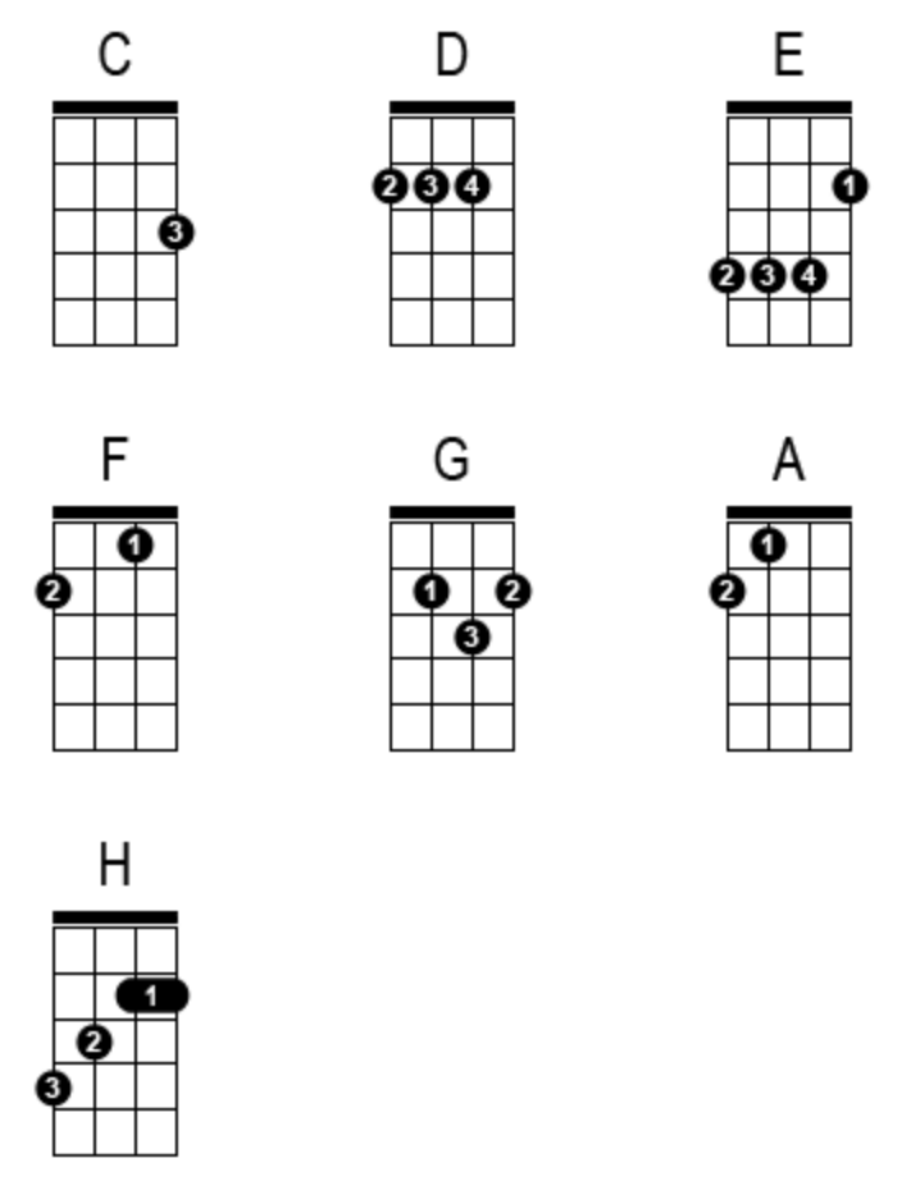
\includegraphics[width=0.25\linewidth]{../images/acc01_dur}
\hfill
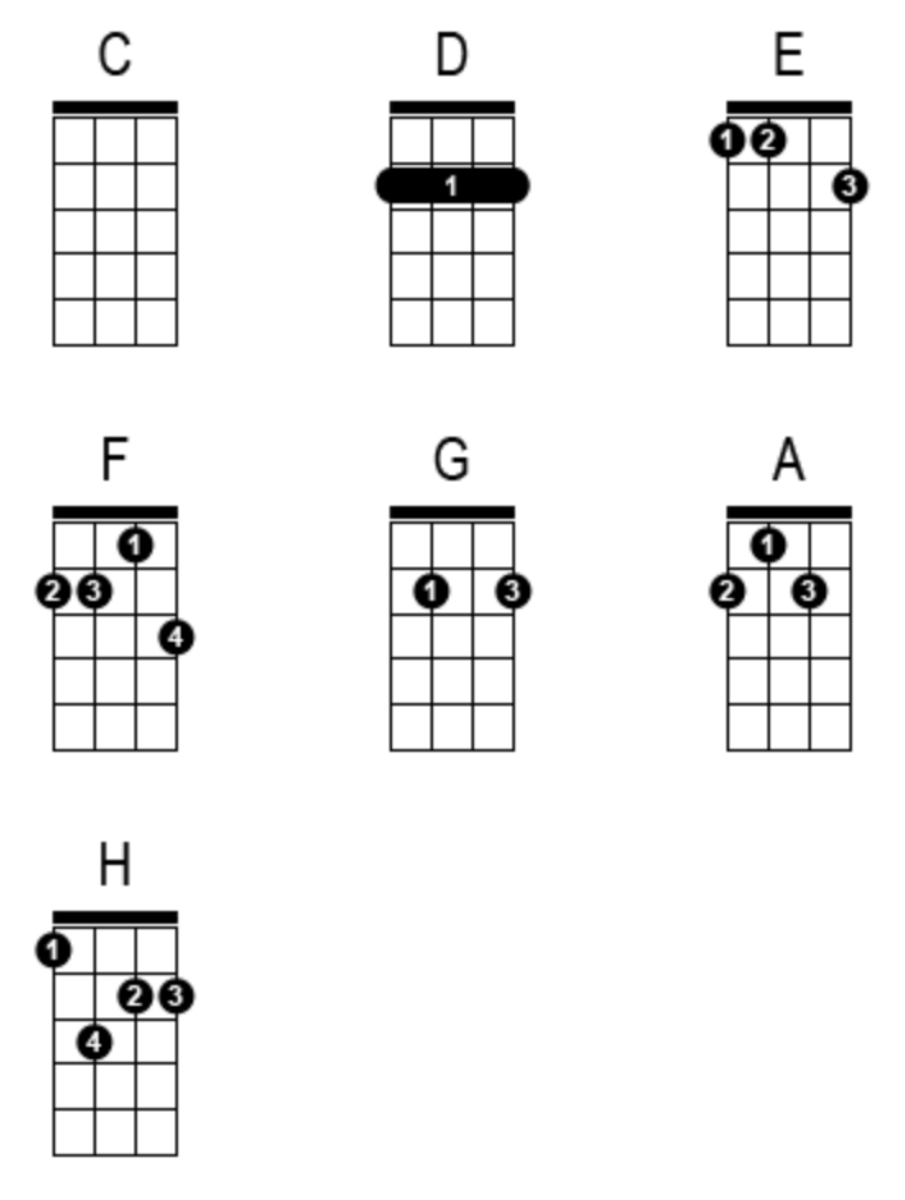
\includegraphics[width=0.25\linewidth]{../images/acc02_6}
\hfill
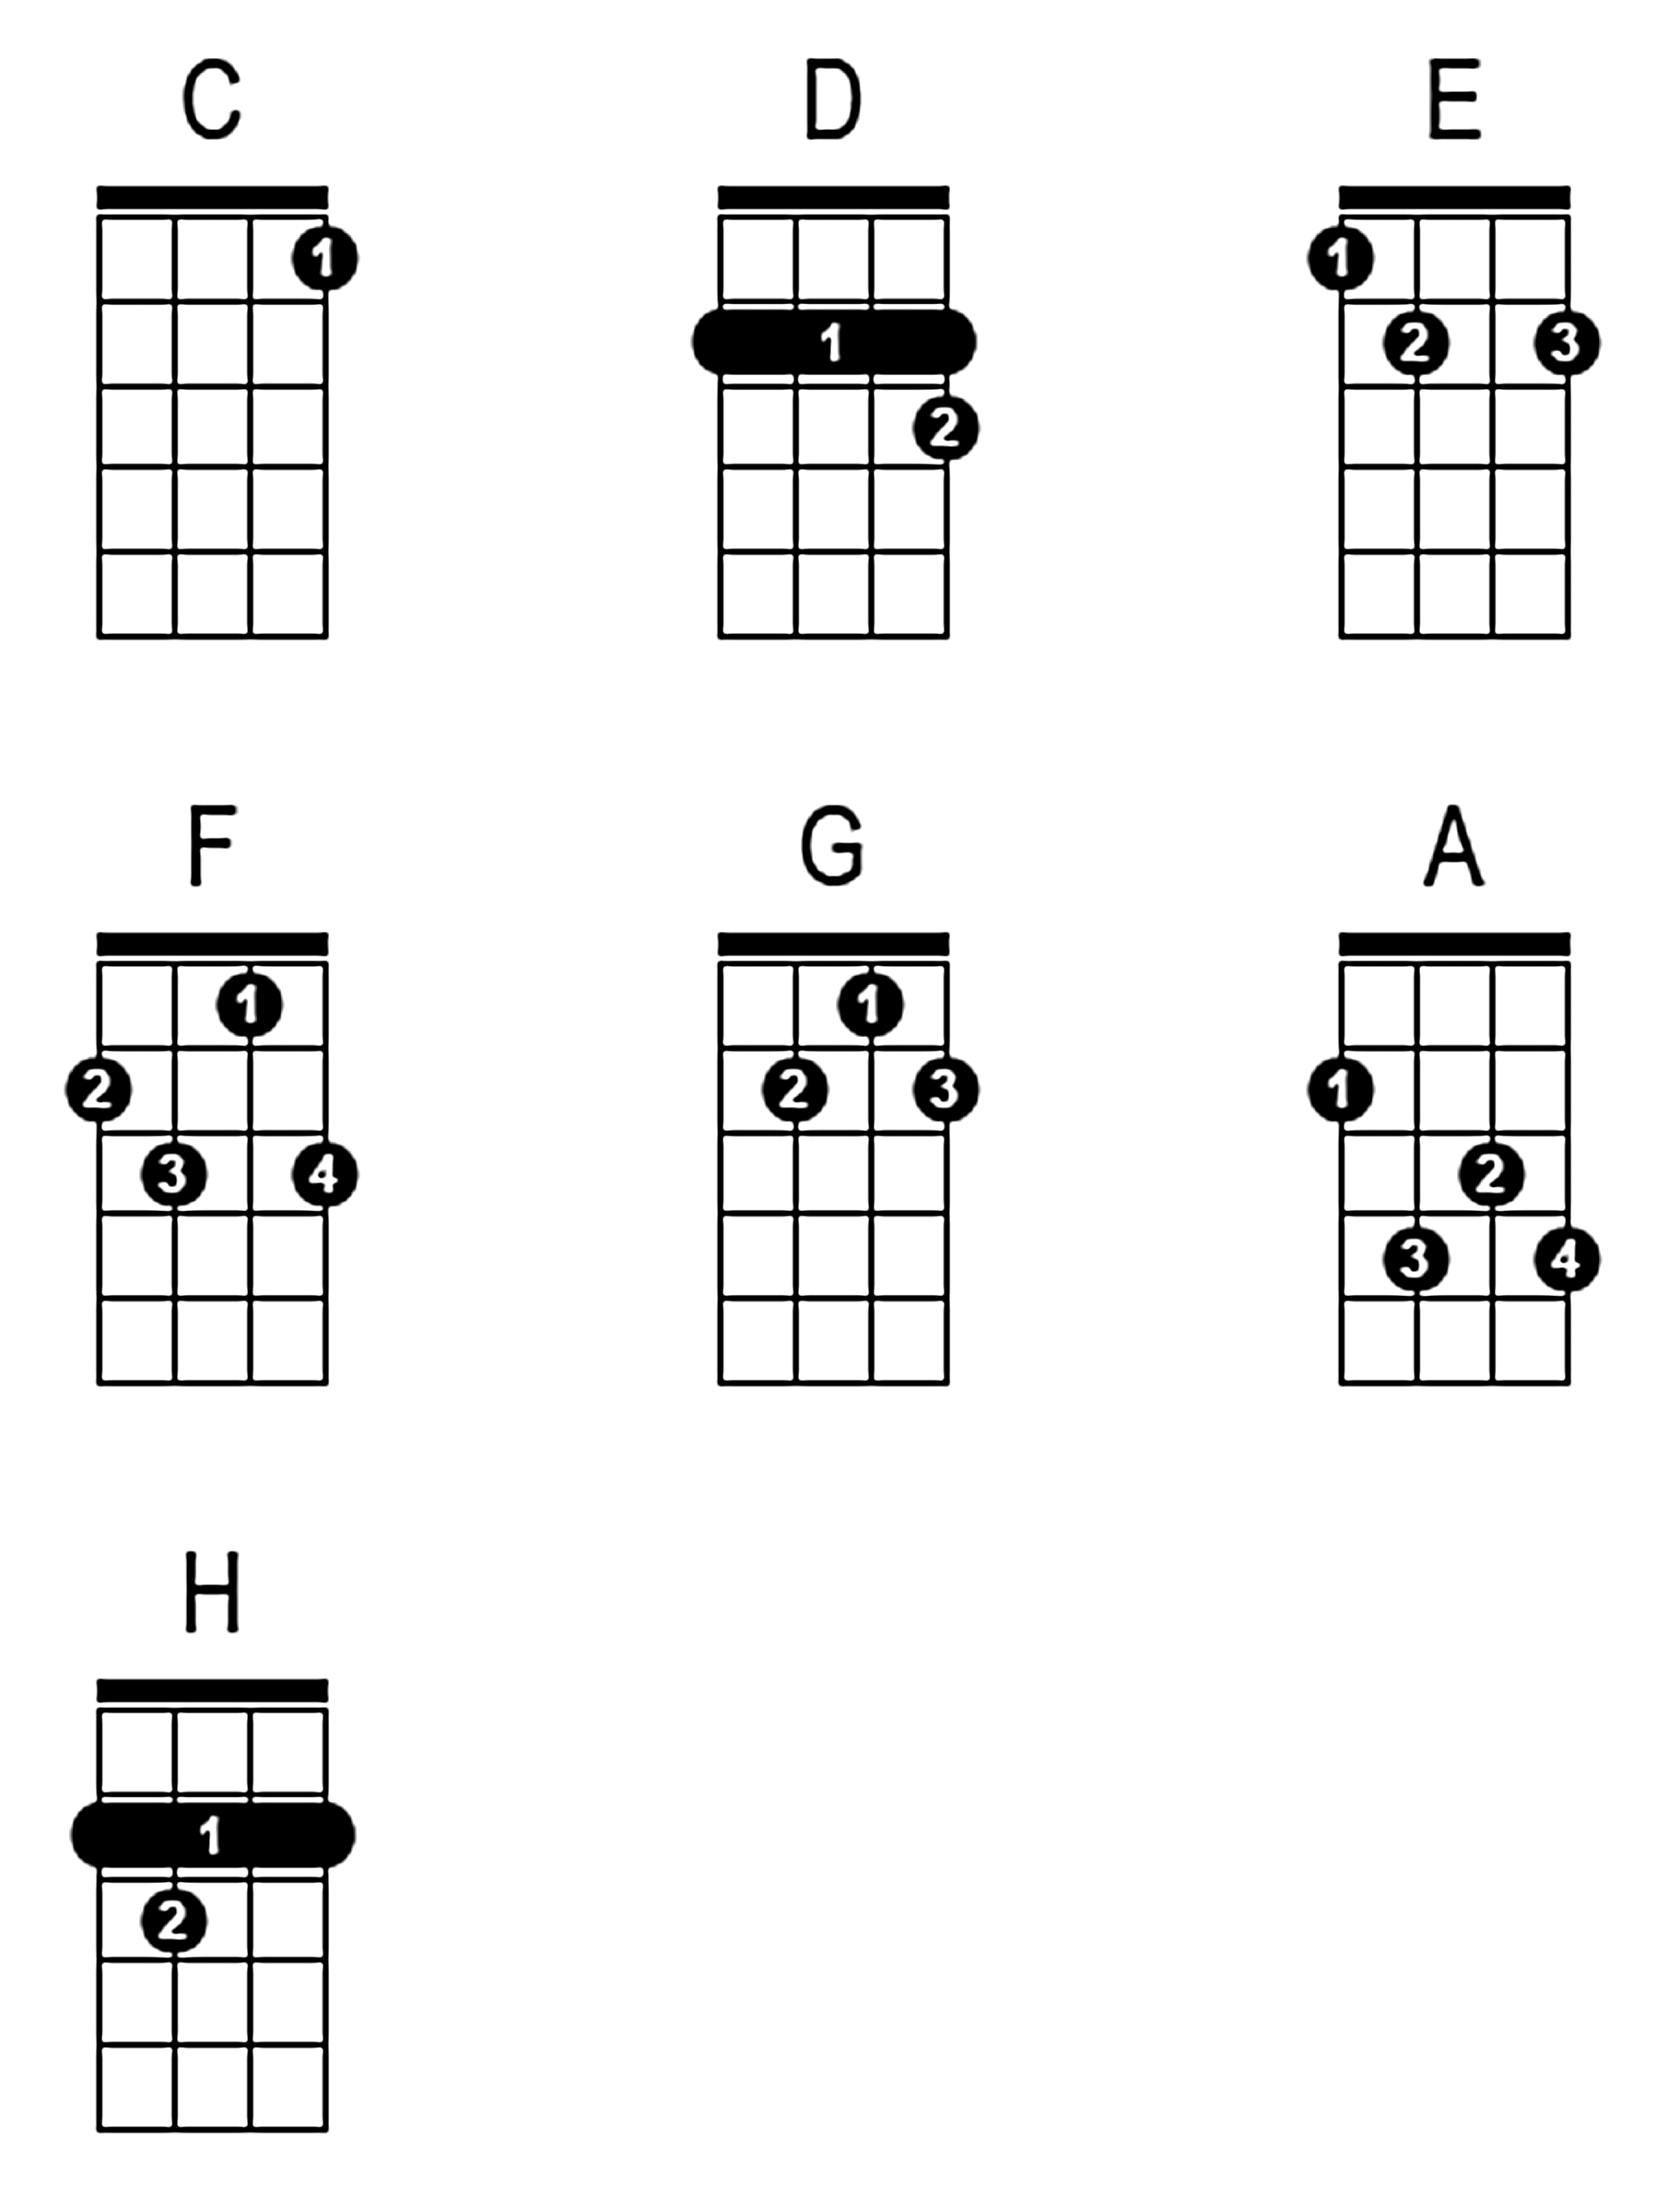
\includegraphics[width=0.25\linewidth]{../images/acc03_7}
\hfill\\
%
~\\~\\~\\~\\~\\
%
\makebox[\textwidth][s]{\textit{~~moll ~~~~ m6 ~~~~ m7~~}}\\~\\~\\
%
\noindent\hfill
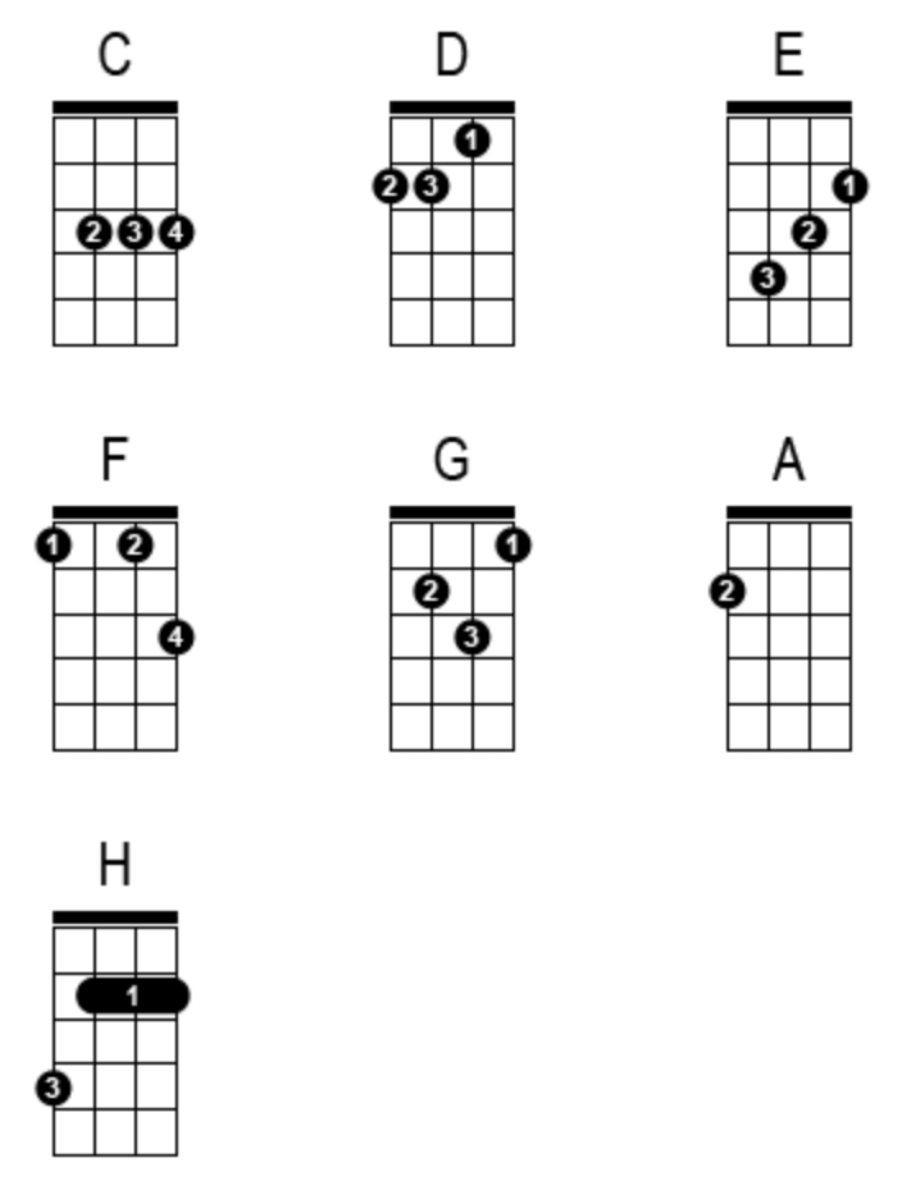
\includegraphics[width=0.25\linewidth]{../images/acc04_moll}
\hfill
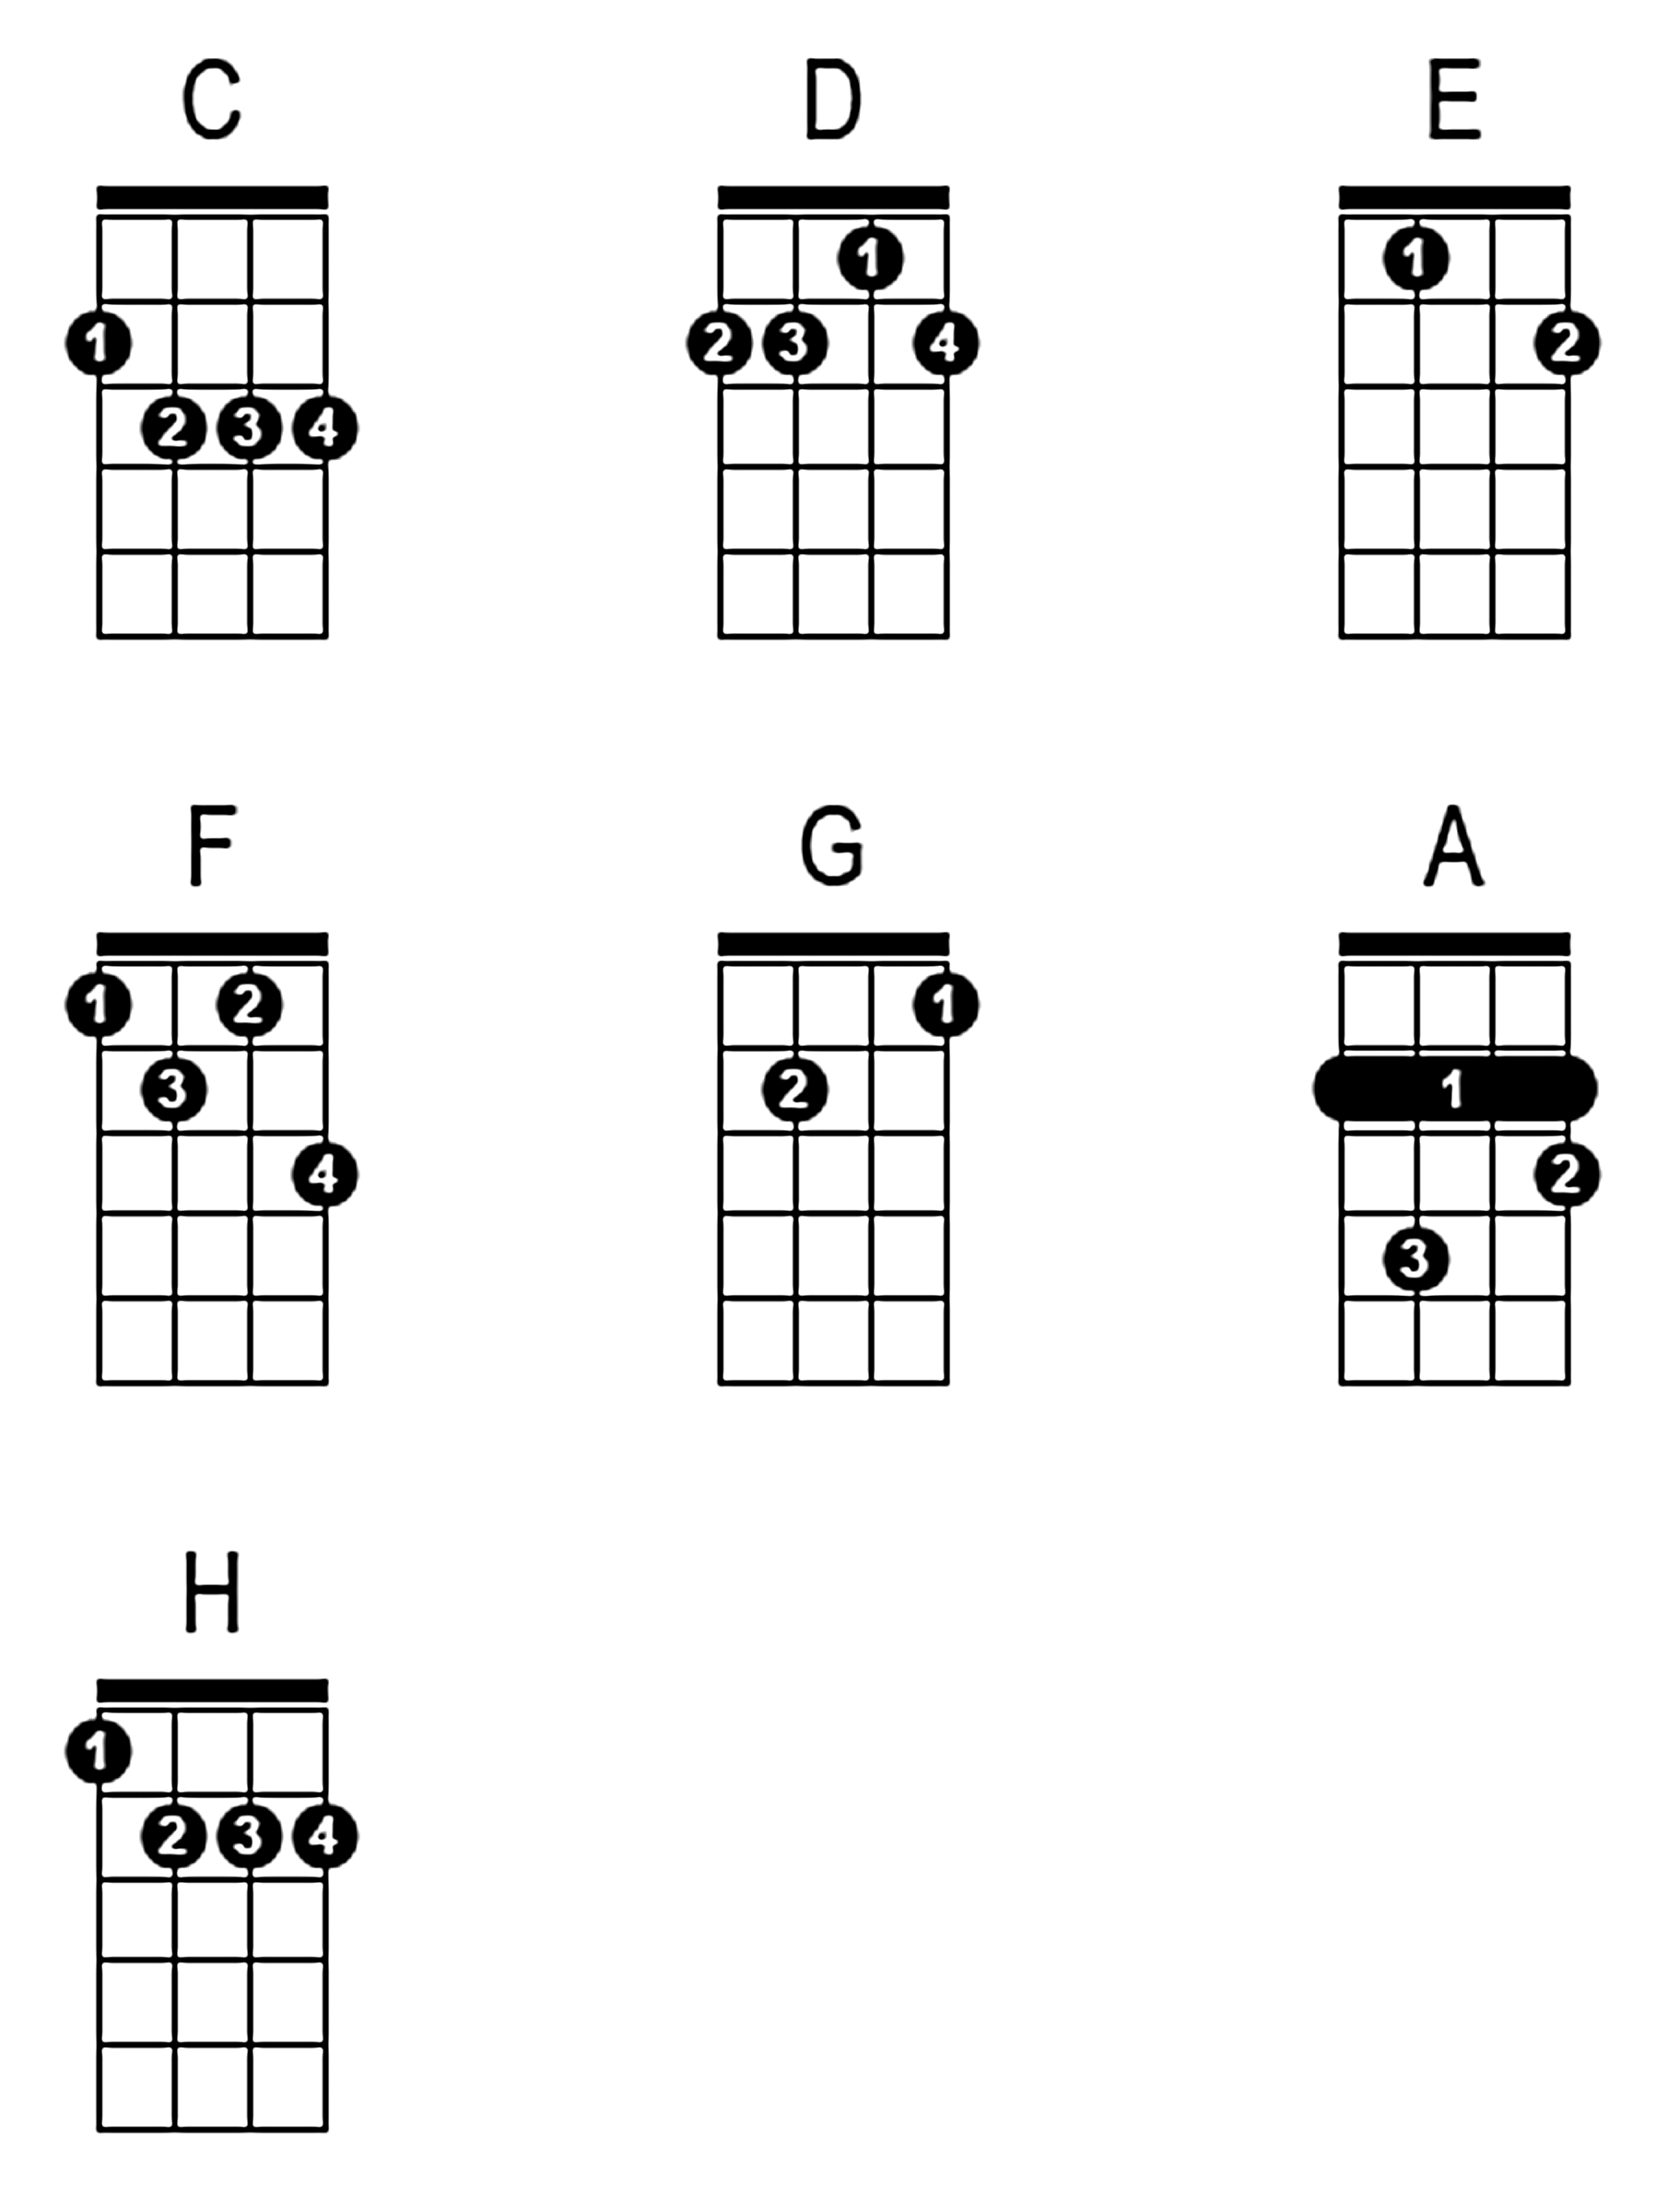
\includegraphics[width=0.25\linewidth]{../images/acc05_m6}
\hfill
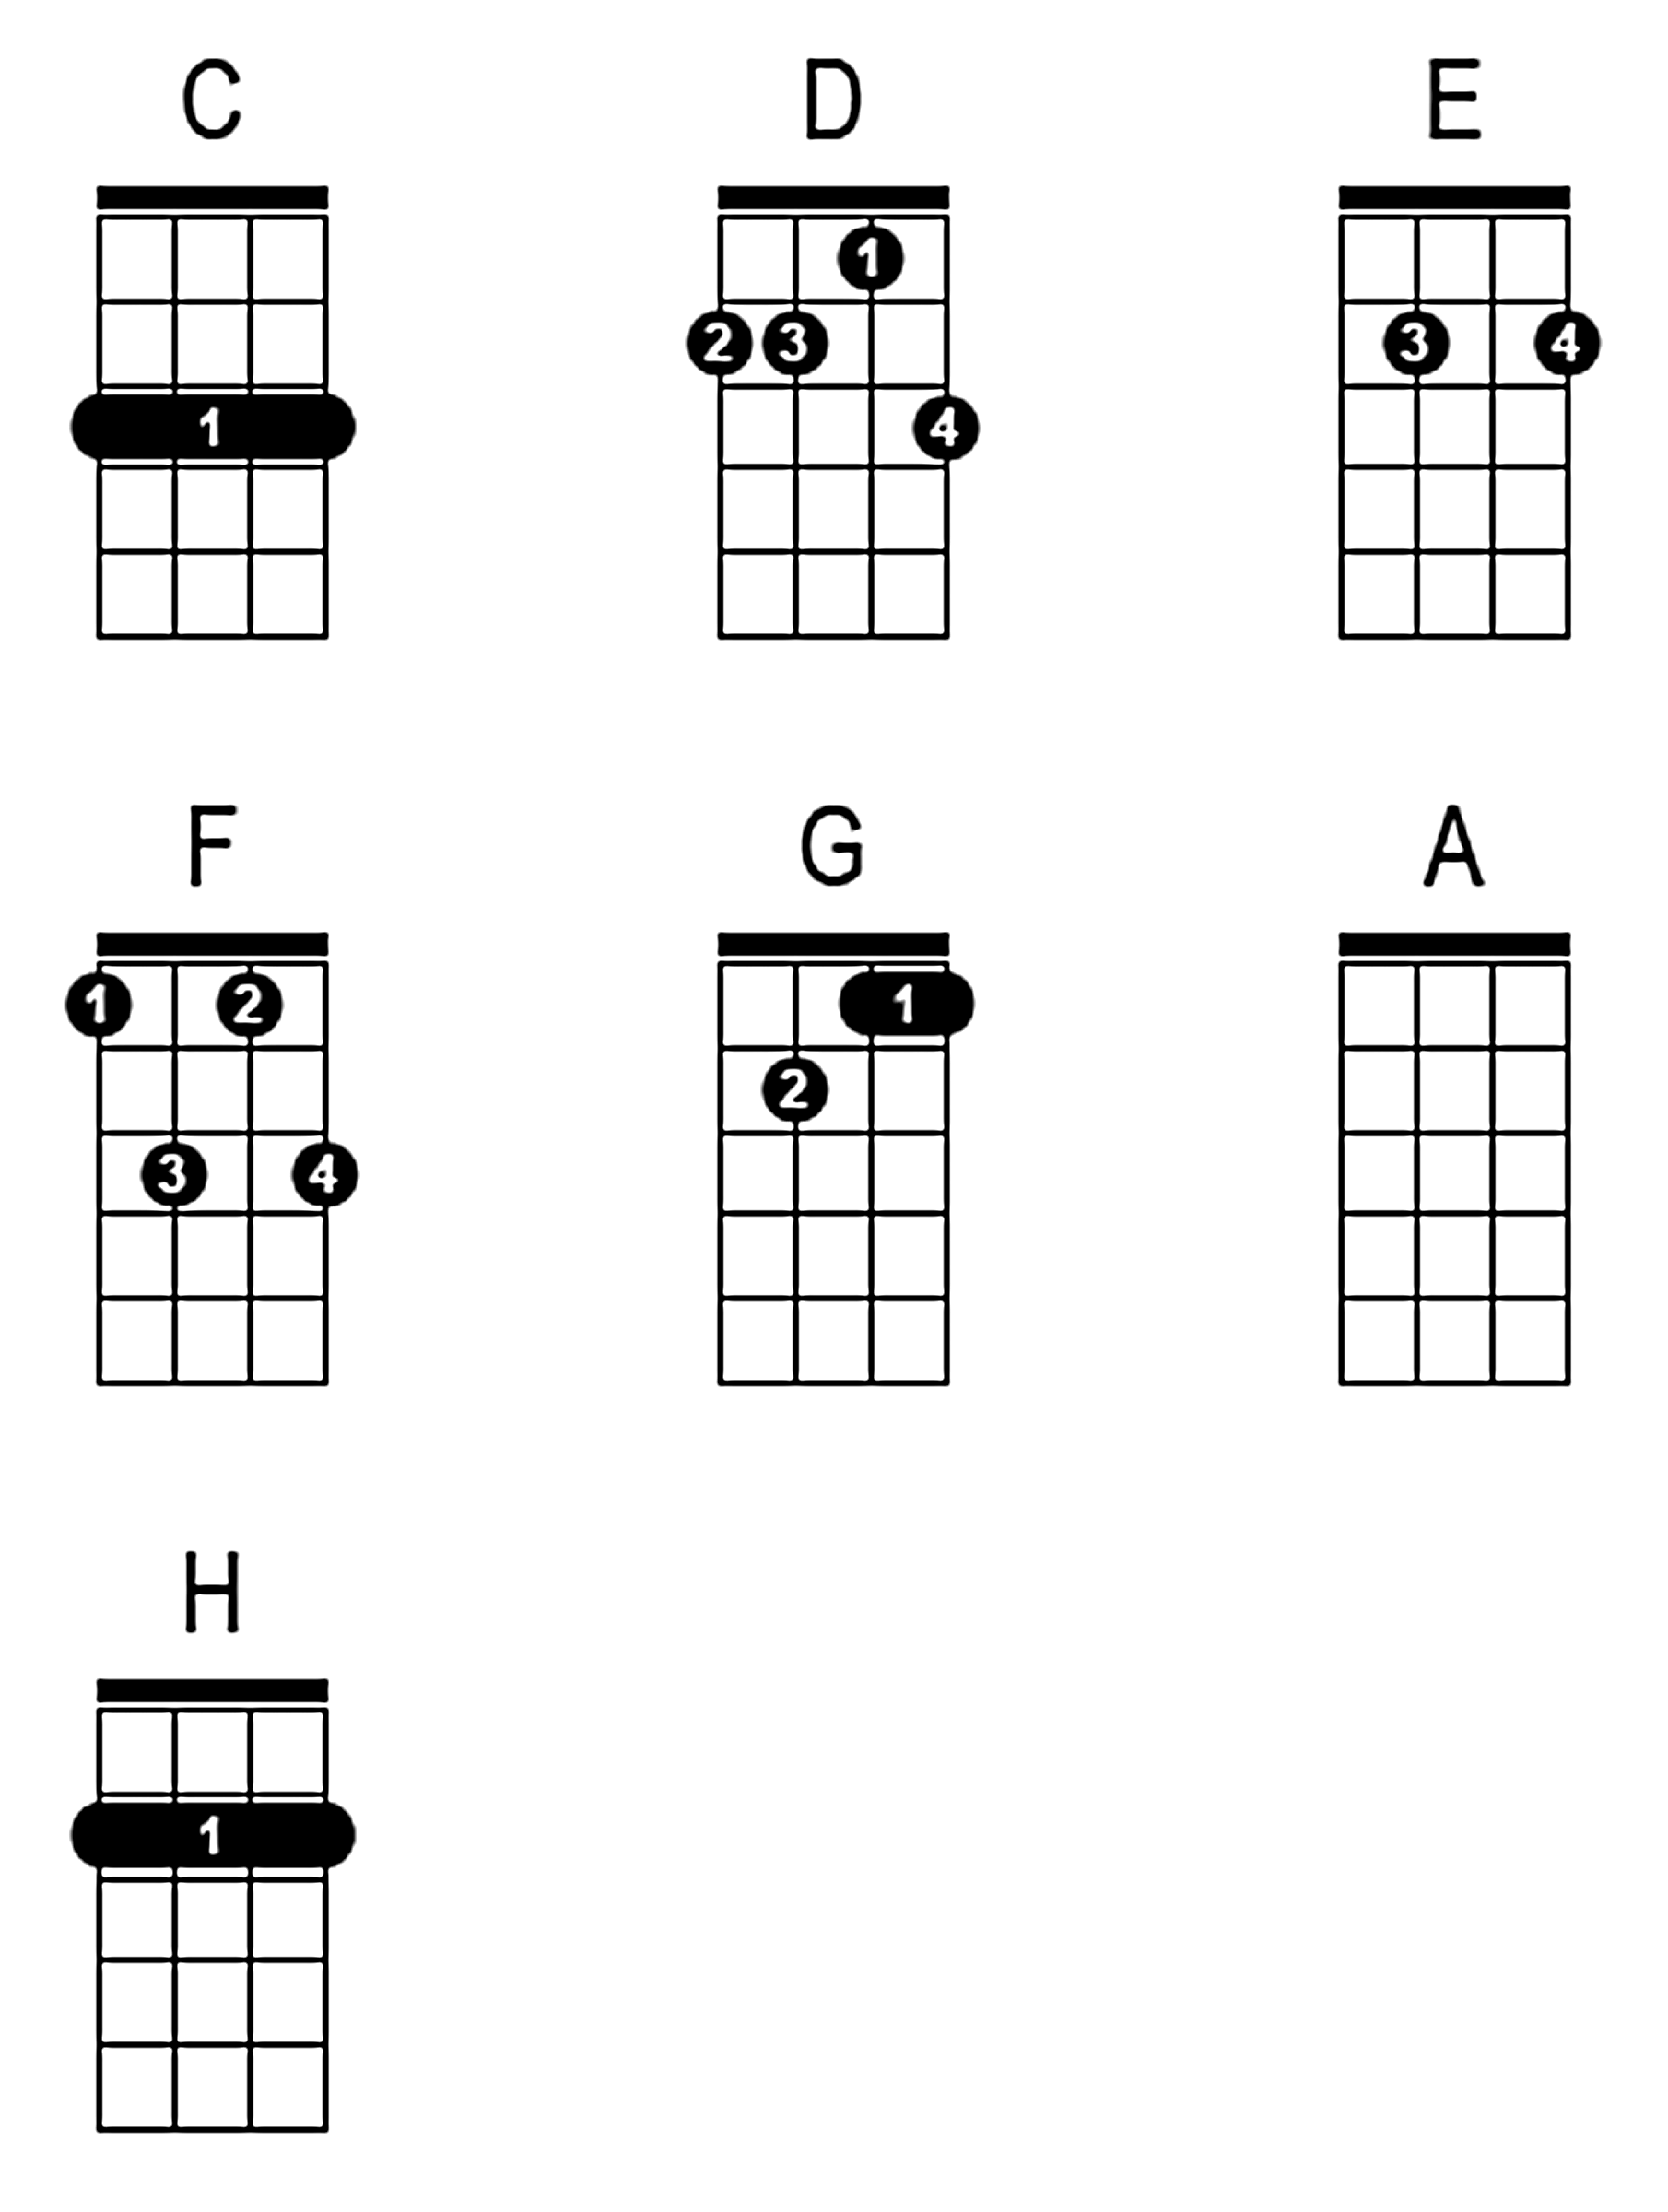
\includegraphics[width=0.25\linewidth]{../images/acc06_m7}
\hfill\\%
%
~\\~\\~\\~\\~\\
%
\makebox[\textwidth][s]{\textit{~sus2 ~ sus4 ~ Maj7 ~ Dim7~}}\\~\\~\\
%
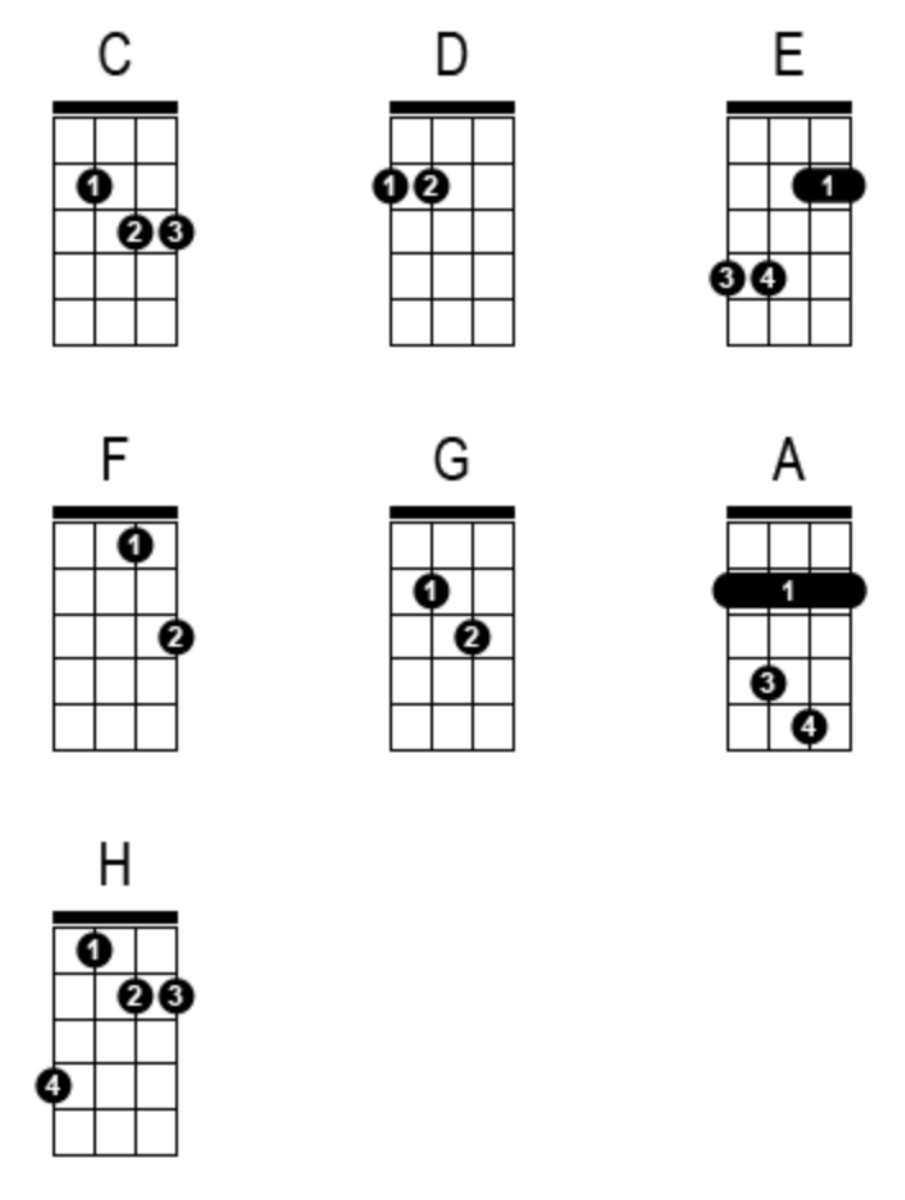
\includegraphics[width=0.2\linewidth]{../images/acc07_sus2}
\hfill
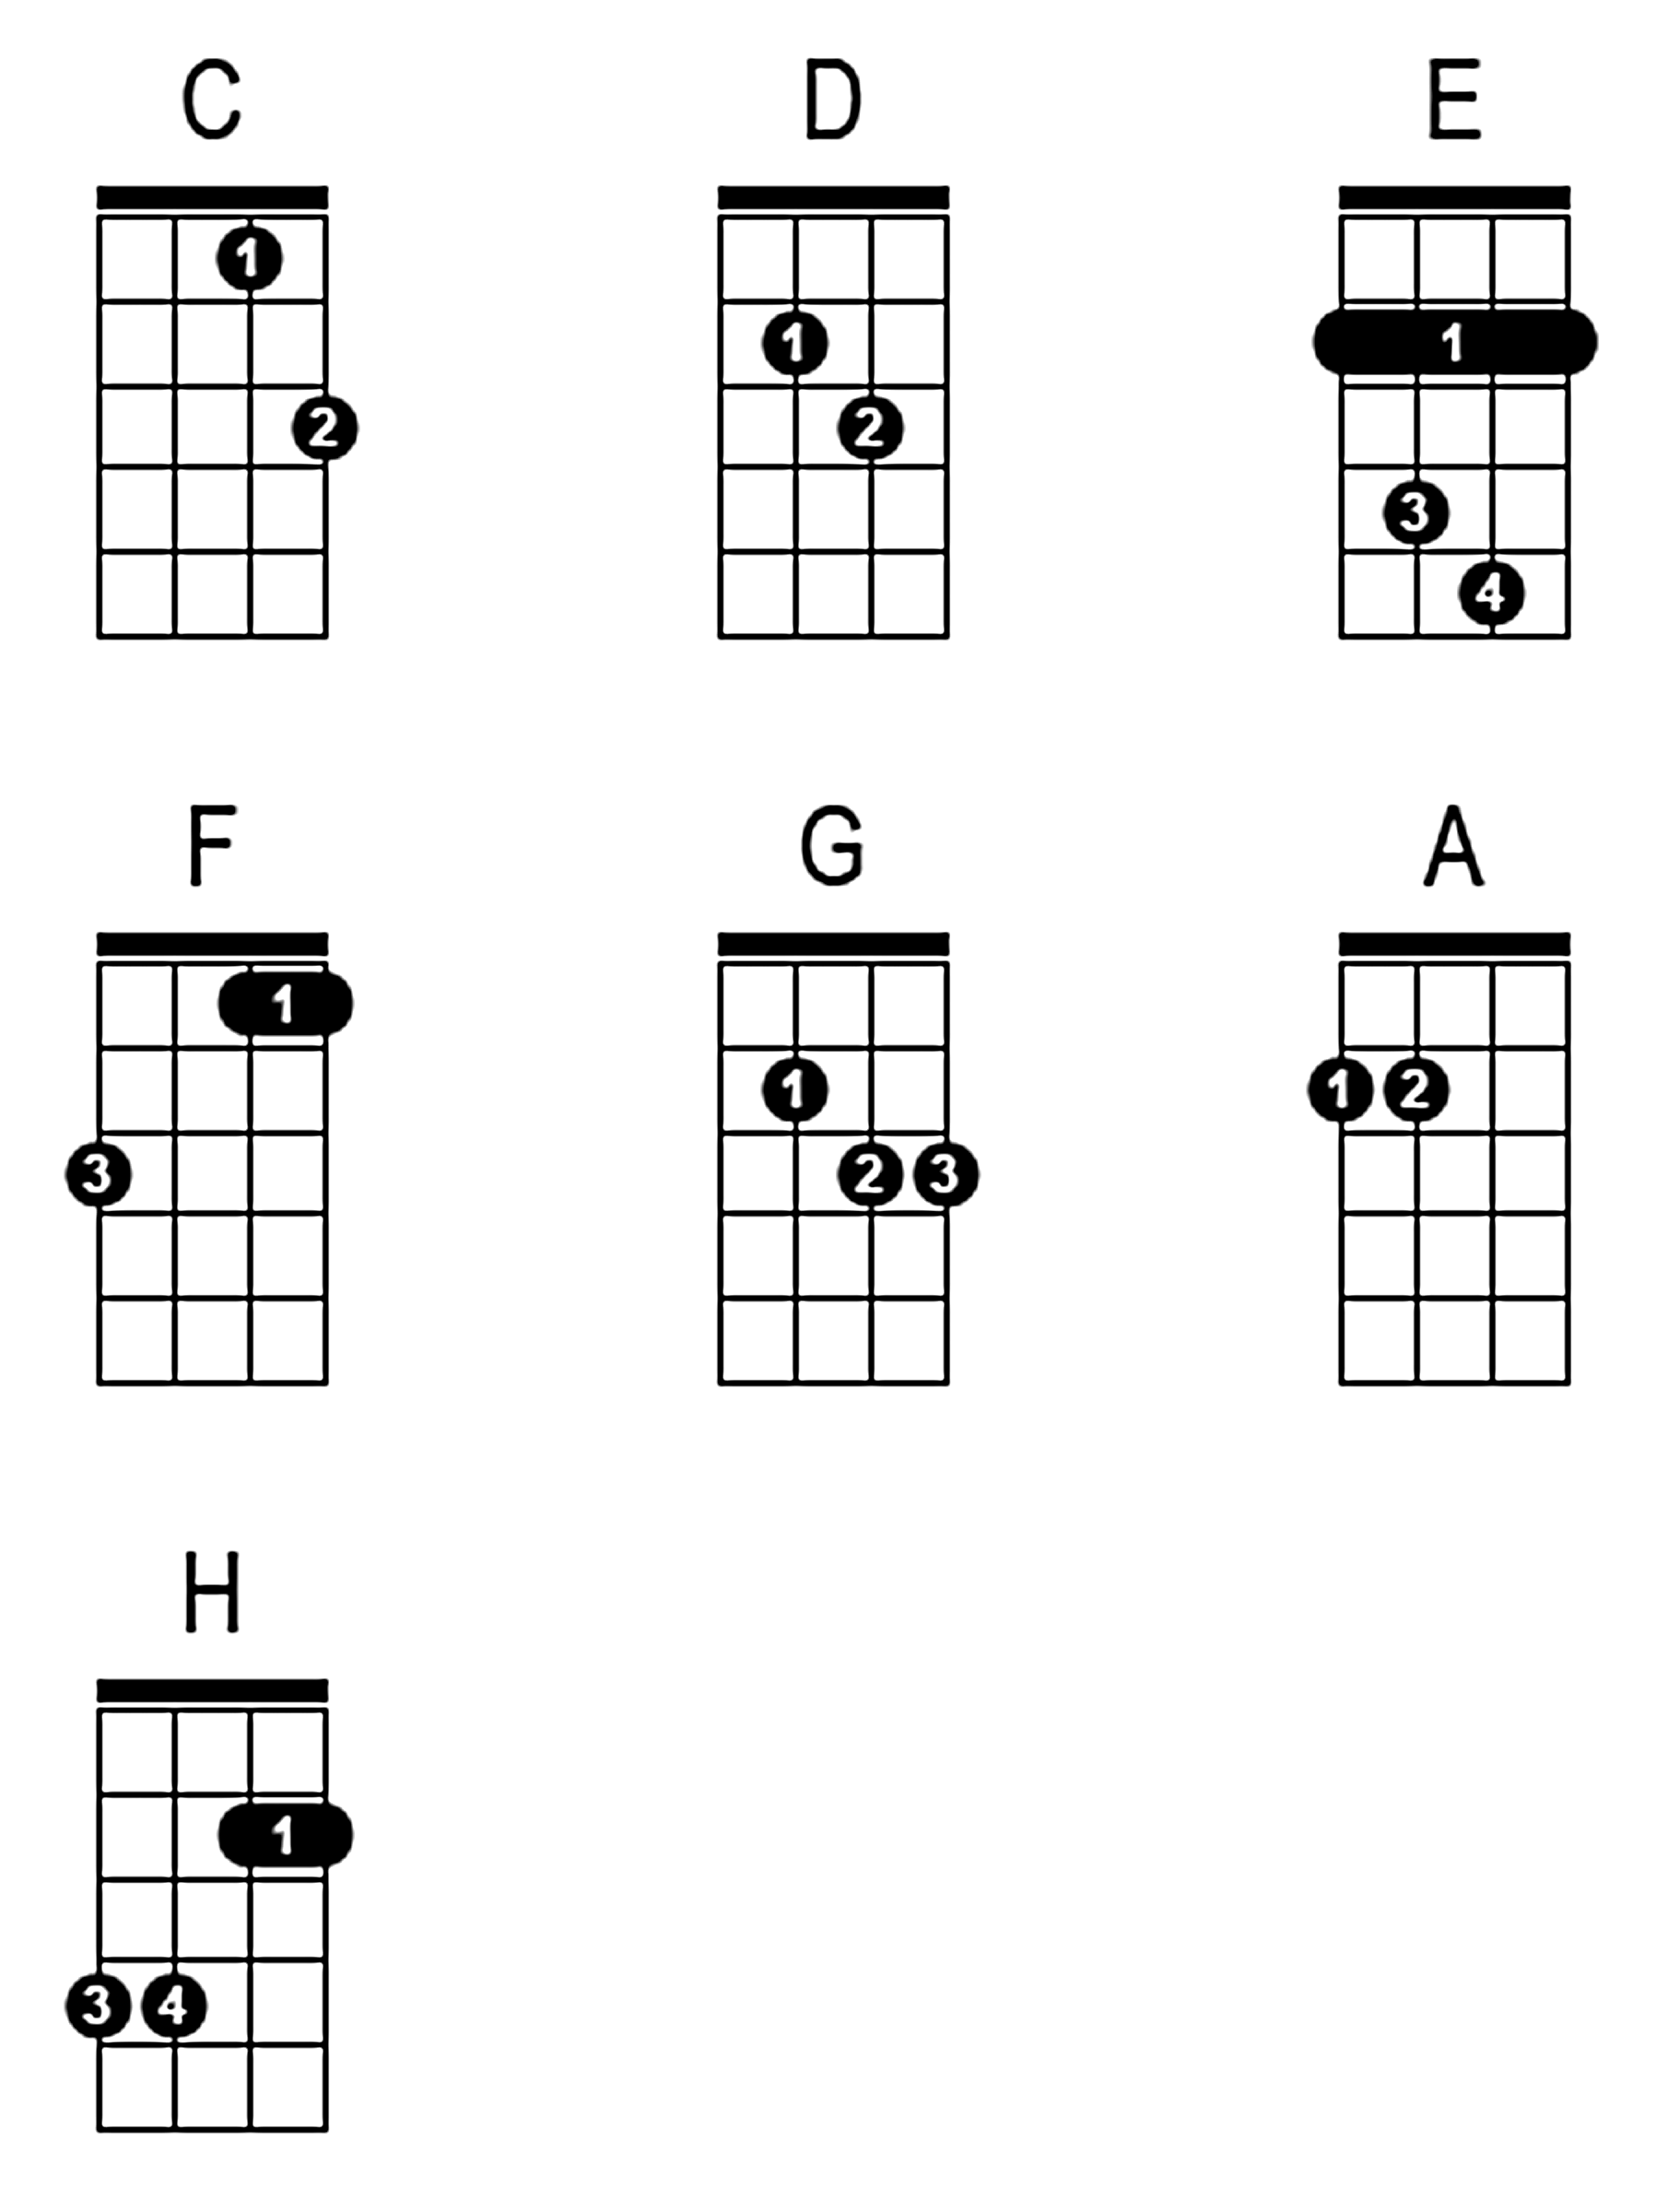
\includegraphics[width=0.2\linewidth]{../images/acc08_sus4}
\hfill
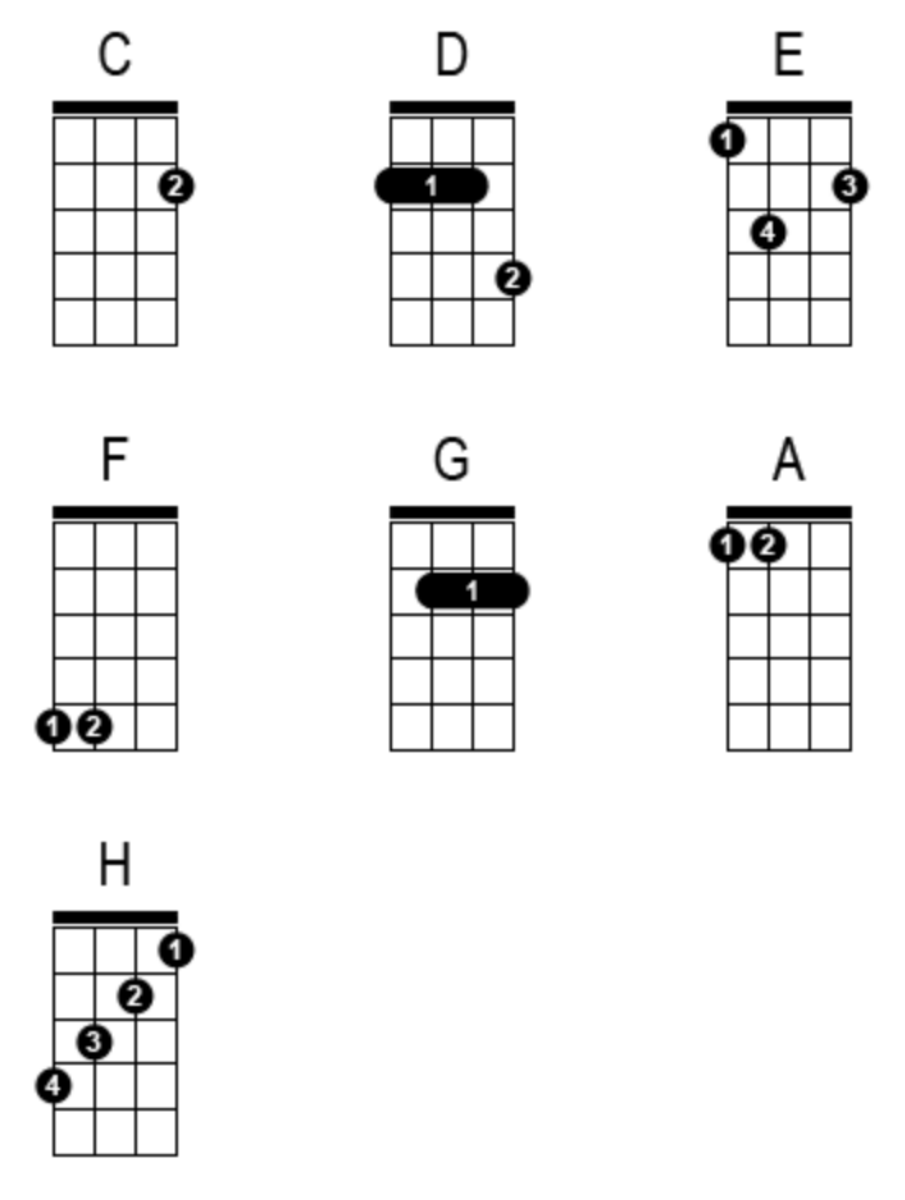
\includegraphics[width=0.2\linewidth]{../images/acc09_Maj7}
\hfill
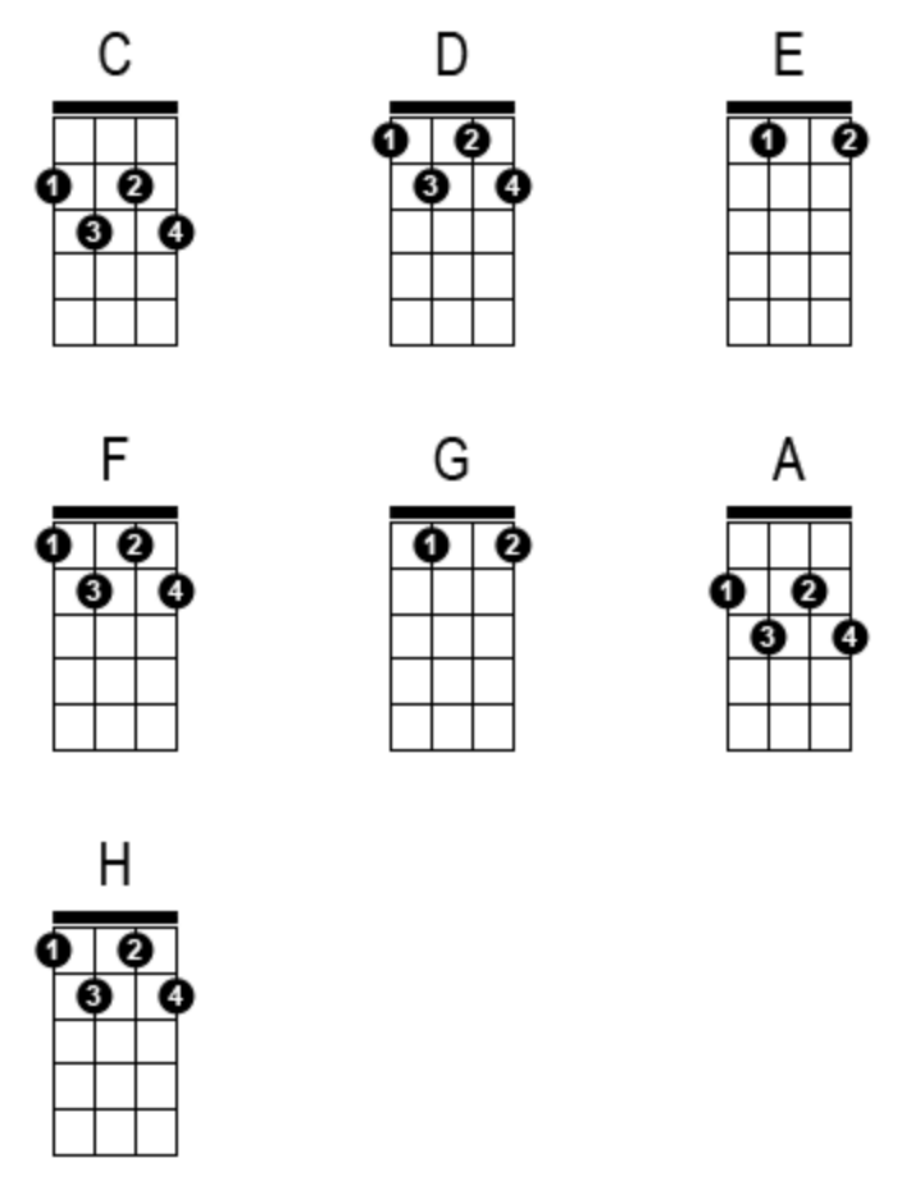
\includegraphics[width=0.2\linewidth]{../images/acc10_Dim7}
%\hfill

\clearpage
%\drawukulelechord{2,1,0,0}
\hspace{-2.5cm}%
\renewcommand{\arraystretch}{3.5}
%  copied from here: https://tex.stackexchange.com/questions/318670/generating-ukulele-chord-diagrams
\begin{tabular}{r|ccccccccccccc}
	         & maj                        & 6                           & 7                           & 9                           & maj7                        & m                           & m6                          & m7                          & m9                          & sus2                        & sus4                        & +                           & dim                         \\\hline
	C        & \drawukulelechord{0,0,0,3} & \drawukulelechord{0,0,0,0} & \drawukulelechord{0,0,0,1} & \drawukulelechord{0,2,0,1} & \drawukulelechord{0,0,0,2} & \drawukulelechord{0,3,3,3} & \drawukulelechord{0,3,3,0} & \drawukulelechord{3,3,3,3} & \drawukulelechord{5,3,3,5} & \drawukulelechord{0,2,3,3} & \drawukulelechord{0,0,1,3} & \drawukulelechord{1,0,0,3} & \drawukulelechord{2,3,2,3} \\
	\shortstack[r]{C\# \\\vspace{-0.5cm}/ Db} & \drawukulelechord{1,1,1,4} & \drawukulelechord{1,1,1,1} & \drawukulelechord{1,1,1,2} & \drawukulelechord{1,3,1,2} & \drawukulelechord{1,1,1,3} & \drawukulelechord{5,3,3,3} & \drawukulelechord{1,4,4,1} & \drawukulelechord{1,4,4,2} & \drawukulelechord{1,3,0,4} & \drawukulelechord{1,3,4,4} & \drawukulelechord{1,1,2,4} & \drawukulelechord{2,1,1,0} & \drawukulelechord{0,1,0,1} \\
	D        & \drawukulelechord{2,2,2,0} & \drawukulelechord{2,2,2,2} & \drawukulelechord{2,2,2,3} & \drawukulelechord{2,4,2,3} & \drawukulelechord{2,2,2,4} & \drawukulelechord{2,2,1,0} & \drawukulelechord{2,2,1,2} & \drawukulelechord{2,2,1,3} & \drawukulelechord{2,4,1,5} & \drawukulelechord{2,2,0,0} & \drawukulelechord{0,2,3,0} & \drawukulelechord{3,2,2,1} & \drawukulelechord{1,2,1,2} \\
	\shortstack[r]{D\# \\\vspace{-0.5cm}/ Eb} & \drawukulelechord{0,3,3,1} & \drawukulelechord{3,3,3,3} & \drawukulelechord{3,3,3,4} & \drawukulelechord{0,1,1,1} & \drawukulelechord{3,3,3,5} & \drawukulelechord{3,3,2,1} & \drawukulelechord{3,0,2,1} & \drawukulelechord{3,1,2,1} & \drawukulelechord{3,5,2,6} & \drawukulelechord{3,3,1,1} & \drawukulelechord{1,3,4,1} & \drawukulelechord{0,3,3,2} & \drawukulelechord{2,3,2,3} \\
	E        & \drawukulelechord{4,4,4,2} & \drawukulelechord{1,1,0,2} & \drawukulelechord{1,2,0,2} & \drawukulelechord{1,2,2,2} & \drawukulelechord{1,3,0,2} & \drawukulelechord{0,4,3,2} & \drawukulelechord{4,4,3,4} & \drawukulelechord{0,2,0,2} & \drawukulelechord{0,4,2,2} & \drawukulelechord{4,4,2,2} & \drawukulelechord{2,4,5,2} & \drawukulelechord{1,0,0,3} & \drawukulelechord{0,1,0,1} \\
	F        & \drawukulelechord{2,0,1,0} & \drawukulelechord{2,2,1,3} & \drawukulelechord{2,3,1,0} & \drawukulelechord{2,3,3,3} & \drawukulelechord{2,4,1,3} & \drawukulelechord{1,0,1,3} & \drawukulelechord{1,2,1,3} & \drawukulelechord{1,3,1,3} & \drawukulelechord{0,5,4,3} & \drawukulelechord{0,0,1,3} & \drawukulelechord{3,0,1,1} & \drawukulelechord{2,1,1,0} & \drawukulelechord{1,2,1,2} \\
	\shortstack[r]{F\# \\\vspace{-0.5cm}/ Gb} & \drawukulelechord{3,1,2,1} & \drawukulelechord{3,3,1,4} & \drawukulelechord{3,4,2,0} & \drawukulelechord{1,1,0,1} & \drawukulelechord{3,5,2,4} & \drawukulelechord{2,1,2,0} & \drawukulelechord{2,3,2,4} & \drawukulelechord{2,4,2,4} & \drawukulelechord{1,1,2,0} & \drawukulelechord{1,1,2,4} & \drawukulelechord{4,2,3,3} & \drawukulelechord{3,2,2,1} & \drawukulelechord{2,3,2,3} \\
	G        & \drawukulelechord{0,2,3,2} & \drawukulelechord{0,2,0,2} & \drawukulelechord{0,2,1,2} & \drawukulelechord{2,2,1,2} & \drawukulelechord{0,2,2,2} & \drawukulelechord{0,2,3,1} & \drawukulelechord{0,2,0,1} & \drawukulelechord{0,2,1,1} & \drawukulelechord{2,2,3,1} & \drawukulelechord{0,2,3,0} & \drawukulelechord{0,2,3,3} & \drawukulelechord{0,3,3,2} & \drawukulelechord{0,1,0,1} \\
	\shortstack[r]{G\# \\\vspace{-0.5cm}/ Ab} & \drawukulelechord{5,3,4,3} & \drawukulelechord{1,3,1,3} & \drawukulelechord{1,3,2,3} & \drawukulelechord{3,3,2,3} & \drawukulelechord{1,3,3,3} & \drawukulelechord{4,3,4,2} & \drawukulelechord{1,3,1,2} & \drawukulelechord{1,3,2,2} & \drawukulelechord{3,3,4,2} & \drawukulelechord{1,3,4,1} & \drawukulelechord{1,3,4,4} & \drawukulelechord{1,0,0,3} & \drawukulelechord{1,2,1,2} \\
	A        & \drawukulelechord{2,1,0,0} & \drawukulelechord{2,1,2,0} & \drawukulelechord{0,1,0,0} & \drawukulelechord{0,1,0,2} & \drawukulelechord{1,1,0,0} & \drawukulelechord{2,0,0,0} & \drawukulelechord{2,0,2,0} & \drawukulelechord{0,0,0,0} & \drawukulelechord{2,0,0,2} & \drawukulelechord{2,4,5,2} & \drawukulelechord{2,2,0,0} & \drawukulelechord{2,1,1,0} & \drawukulelechord{2,3,2,3} \\
	\shortstack[r]{A\# \\\vspace{-0.5cm}/ B}  & \drawukulelechord{3,2,1,1} & \drawukulelechord{0,2,1,1} & \drawukulelechord{1,2,1,1} & \drawukulelechord{1,2,1,3} & \drawukulelechord{3,2,1,0} & \drawukulelechord{3,1,1,1} & \drawukulelechord{3,1,3,1} & \drawukulelechord{1,1,1,1} & \drawukulelechord{3,1,1,3} & \drawukulelechord{3,0,1,1} & \drawukulelechord{3,3,1,1} & \drawukulelechord{3,2,2,1} & \drawukulelechord{0,1,0,1} \\
	H        & \drawukulelechord{4,3,2,2} & \drawukulelechord{1,3,2,2} & \drawukulelechord{2,3,2,2} & \drawukulelechord{2,3,2,4} & \drawukulelechord{4,3,2,1} & \drawukulelechord{4,2,2,2} & \drawukulelechord{1,2,2,2} & \drawukulelechord{2,2,2,2} & \drawukulelechord{4,2,2,4} & \drawukulelechord{4,1,2,2} & \drawukulelechord{4,4,2,2} & \drawukulelechord{0,3,3,2} & \drawukulelechord{1,2,1,2}
\end{tabular}

\end{document}



